\section{Backend Service Architecture}
\label{sec:backend-service-architecture}

The Stockrium backend is the authoritative application boundary between the mobile and administrative clients and the project's financial data, user records, and AI workflows. It is implemented as a FastAPI application served by Uvicorn. In addition to exposing HTTP endpoints, the backend validates input, establishes the authenticated user context, applies domain rules, normalizes heterogeneous data, invokes analytical workflows, and converts results into client-oriented response objects. This concentration of authority prevents the mobile application from directly accessing database credentials, market-provider credentials, or language-model keys.

The implementation is organized primarily into route, model, service, and utility or infrastructure-client modules. This organization is deliberately lightweight: the project does not introduce a repository class for every database table, while database and external-service access is primarily separated from presentation logic and grouped with the domain service that owns the corresponding operation. The resulting structure provides clear responsibility boundaries without adding abstractions that would contribute little to the current application size.

\subsection{FastAPI Layered Design}
\label{subsec:fastapi-layered-design}

FastAPI constructs the Hypertext Transfer Protocol (HTTP) interface from typed Python endpoint declarations and integrates Pydantic validation and OpenAPI schema generation \cite{fastapiFeatures2026}. Stockrium uses these capabilities to establish a layered request path. Figure~\ref{fig:backend-layered-design} shows the logical direction of a normal backend call. A request enters through either the mobile application or the internal administrative web application. It then passes through cross-cutting HTTP behavior, an application programming interface (API) router, a typed model where applicable, and a domain service. The service can query persisted data, call an upstream provider, perform deterministic computation, or invoke an agent graph.

\begin{figure}[H]
    \centering
    \IfFileExists{figures/chapter4/stockrium_backend_layered_design.png}{%
        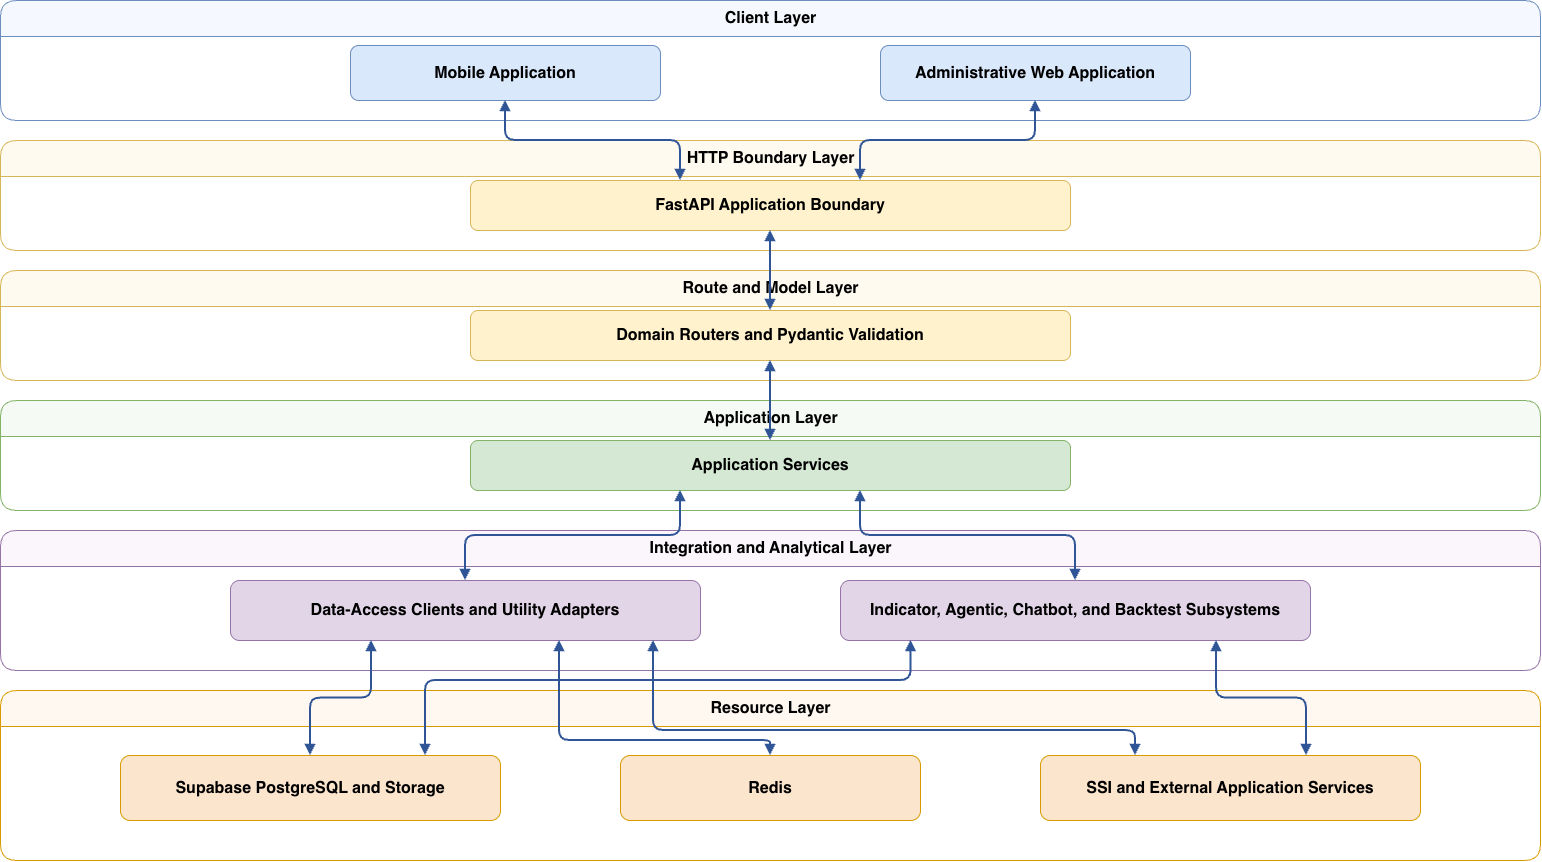
\includegraphics[width=\textwidth,height=0.78\textheight,keepaspectratio]{figures/chapter4/stockrium_backend_layered_design.png}%
    }{%
        \fbox{\parbox[c][5.5cm][c]{0.92\textwidth}{\centering
        Export the Draw.io diagram as\\
        \texttt{figures/chapter4/stockrium\_backend\_layered\_design.png}}}%
    }
    \caption{Layered design of the Stockrium backend service}
    \label{fig:backend-layered-design}
\end{figure}

The layers in Figure~\ref{fig:backend-layered-design} have the following responsibilities:

\begin{itemize}
    \item \textbf{Application boundary.} The FastAPI application registers routers, configures Cross-Origin Resource Sharing (CORS) for allowed browser origins, exposes health endpoints, mounts generated backtest visualizations, and installs common exception handlers. Configuration is loaded from typed environment settings so deployment-specific addresses and credentials are not embedded in route code.
    \item \textbf{Route layer.} Route modules define URL paths, HTTP methods, query and body parameters, access dependencies, and response construction. They remain relatively thin: a route extracts validated values, calls a service, and translates a domain or infrastructure failure into an HTTP result.
    \item \textbf{Model layer.} Pydantic classes describe input and output structures. Once validation succeeds, services receive typed objects rather than unstructured request dictionaries \cite{pydanticModels2026}. These models are particularly important for configurable artificial intelligence (AI) analysis, manual weights, investment-horizon records, authentication, and backtest parameters.
    \item \textbf{Service layer.} Services implement application operations such as obtaining a price series, searching stocks, retrieving financial statements, managing a watchlist entry, calculating technical indicators, running an analysis graph, or maintaining a chat session. A service may combine several tables or providers into one response suited to a user task.
    \item \textbf{Utility and infrastructure layer.} Supabase clients, the direct PostgreSQL connection pool, Redis session operations, SSI FastConnect market-data access, email and Google Identity utilities, model software development kits (SDKs), and Supabase Storage helpers isolate protocol-specific interactions from HTTP routing.
\end{itemize}

This flow is visible in a technical-indicator request. The protected route first obtains the current user from the authentication dependency and validates the requested interval. The market service loads an ordered price series for the symbol, and pandas represents and transforms it as a DataFrame. The technical-indicator service uses the Technical Analysis Library (TA-Lib) to calculate the simple moving average (SMA), exponential moving average (EMA), relative strength index (RSI), moving average convergence divergence (MACD), Bollinger Bands, and stochastic KDJ oscillator. Non-finite warm-up values are converted to \texttt{null} so that the result is valid JavaScript Object Notation (JSON). Finally, the route aligns every indicator value with its trading date and time and returns records suitable for chart rendering. The route does not contain the formulas, and the indicator service does not handle bearer tokens or HTTP status codes.

An AI-analysis request follows the same outer structure but changes at the service boundary. The route validates the analysis configuration and passes the symbol, mode, investment horizon, data-selection switches, and optional weights to the agentic service. The service creates the initial graph state and invokes a compiled LangGraph workflow. Consequently, the HTTP layer is independent of the internal number of specialist agents; later changes to graph routing do not require the mobile request contract to be redesigned.

\subsection{Domain API Modules}
\label{subsec:backend-domain-api-modules}

Routers are divided by application domain instead of by screen. A stock-detail screen can therefore compose calls from the market, company, article, fundamental, and technical modules, while the same modules can be reused by other screens and analytical workflows. Tables~\ref{tab:backend-domain-modules} and~\ref{tab:backend-domain-modules-operational} summarize the modules that belong to the current application.

\begin{table}[htbp]
    \centering
    \caption{Active backend API modules and responsibilities: core data services}
    \label{tab:backend-domain-modules}
    \small
    \setlength{\tabcolsep}{4pt}
    \renewcommand{\arraystretch}{1.22}
    \begin{tabularx}{\textwidth}{>{\raggedright\arraybackslash}p{2.25cm} >{\raggedright\arraybackslash}p{3.35cm} X >{\raggedright\arraybackslash}p{2.45cm}}
        \toprule
        \textbf{Module} & \textbf{Representative interface} & \textbf{Principal responsibility} & \textbf{Main dependency} \\
        \midrule
        Authentication & \texttt{/api/auth/*} & Account creation, email verification, password or Google sign-in, token refresh and revocation, password recovery, and current-user retrieval & Supabase, Redis, Google, Resend \\
        Market and discovery & \texttt{/api/all-stocks}\newline \texttt{/api/price/}\newline \texttt{\{symbol\}}\newline \texttt{/api/market-index}\newline \texttt{/api/investing- idea} & Symbol discovery, current and historical prices, industry movement, index summaries, impact stocks, and deterministic investment-idea lists & Supabase and SSI \\
        Company and fundamentals & \texttt{/api/company/*}\newline \texttt{/api/fundamental-}\newline \texttt{analysis/*} & Company profile, leaders, subsidiaries, financial statements, ratios, stored summaries, and industry aggregates & Supabase \\
        Technical analysis & \texttt{/api/technical-}\newline \texttt{indicators/}\newline \texttt{\{symbol\}} & Load price candles, calculate supported technical-indicator series, align timestamps, and serialize chart-ready values & Market service, pandas, and TA-Lib \\
        Articles & \texttt{/api/articles/*} & Latest, macroeconomic, business, highlighted, category-specific, and stock-specific news retrieval & Supabase \\
        \bottomrule
    \end{tabularx}
\end{table}

\begin{table}[htbp]
    \centering
    \caption{Active backend API modules and responsibilities: user and operational services}
    \label{tab:backend-domain-modules-operational}
    \small
    \setlength{\tabcolsep}{4pt}
    \renewcommand{\arraystretch}{1.22}
    \begin{tabularx}{\textwidth}{>{\raggedright\arraybackslash}p{2.25cm} >{\raggedright\arraybackslash}p{3.35cm} X >{\raggedright\arraybackslash}p{2.45cm}}
        \toprule
        \textbf{Module} & \textbf{Representative interface} & \textbf{Principal responsibility} & \textbf{Main dependency} \\
        \midrule
        Personalization & \texttt{/api/favorite}\newline \texttt{/api/search- history}\newline \texttt{/api/risk- appetite} & User-owned watchlist entries, recent search records, and the selected investment horizon & Supabase and user dependency \\
        Analysis and chat & \texttt{/api/agentic/ analyze}\newline \texttt{/api/agentic/chat}\newline \texttt{/api/agentic/chat/}\newline \texttt{sessions} & Structured stock analysis, stateful conversation, session seeding, history retrieval, and session deletion & LangGraph, model providers, PostgreSQL \\
        Administration and evaluation & \texttt{/api/agentic/}\newline \texttt{admin-analyze}\newline \texttt{/api/agentic/}\newline \texttt{admin-universe/*}\newline \texttt{/api/agentic/ backtest}\newline \texttt{/api/agentic/ backtests} & Role-protected single-symbol or universe analysis, historical pipeline evaluation, and result-artifact listing & Agent graph, backtest services, Supabase Storage \\
        Operations & \texttt{/health}\newline \texttt{/visualizations/*} & Basic process health reporting and delivery of generated backtest visualizations & FastAPI and local artifact directory \\
        \bottomrule
    \end{tabularx}
\end{table}

\FloatBarrier

Authentication is applied through FastAPI dependencies at two levels. Routers containing exclusively protected information---including market, company, fundamental, technical, and article endpoints---declare the current-user dependency once for the entire router. Mixed modules apply the dependency to individual operations. The user dependency verifies the access JSON Web Token (JWT) and also checks that the same token remains present in Redis. This second check enables immediate logout or revocation instead of accepting every cryptographically valid token until its expiry. Administrative operations compose an additional dependency that reads the user's current role from the authoritative \texttt{User} table. A role change therefore takes effect without waiting for a new JWT.

Several services deliberately reuse other domain services. Technical calculation loads candles through the market service instead of implementing a second price-query path. Watchlist and search-history responses enrich stored symbols with profile and current-price information so the mobile client can render useful cards without issuing one request per symbol. Fundamental services resolve a symbol through the \texttt{Stock} relation before obtaining statements and ratios. The agent and chatbot tools also consume the same market, fundamental, technical, and article capabilities used by HTTP routes. Reuse helps keep a value such as the current price or a company identity consistent between a visible screen and an AI response.

\subsection{Request Validation and Response Contract}
\label{subsec:backend-validation-response}

Validation occurs before domain execution whenever an endpoint declares a Pydantic request model. Simple constraints include required fields, numerical bounds, enumerated values, and default settings. Cross-field validation is used when a field cannot be assessed independently. For example, manual AI-analysis weights for news, technical analysis, and fundamental analysis must each be between zero and one, contain no more than two decimal places, and total exactly one after rounding. Backtest parameters bound the maximum holding period, minimum signal score, and lookback window. These checks reduce the chance that invalid configurations reach an expensive model invocation or a long historical simulation.

Validation and normalization are not identical. Pydantic confirms the request shape, while domain services normalize values that carry business meaning. Stock symbols are converted to uppercase before lookup; universe names are stripped and normalized before comparison with \texttt{VN30} and \texttt{VN100}; and Vietnamese chat messages are converted to Unicode Normalization Form C (NFC) before entering the chatbot. The Unicode step is important because visually identical Vietnamese strings can otherwise have different underlying code-point sequences, affecting tokenization, checkpoint content, and comparison behavior.

Client-facing domain endpoints are expected to follow the response envelope shown in Table~\ref{tab:backend-response-envelope}. The envelope separates transport success from the domain payload and gives both clients a stable place to inspect errors. A new universally unique identifier (UUID) is generated for each constructed response. Although the present version does not yet propagate this request identifier through a complete distributed tracing system, it provides a correlation value that can be included in logs and support reports.

\begin{table}[H]
    \centering
    \caption{Standard API response envelope}
    \label{tab:backend-response-envelope}
    \small
    \setlength{\tabcolsep}{6pt}
    \renewcommand{\arraystretch}{1.2}
    \begin{tabular}{p{2.6cm} p{2.3cm} p{7.0cm}}
        \toprule
        \textbf{Field} & \textbf{Type} & \textbf{Meaning} \\
        \midrule
        \texttt{data} & object, array, or scalar & Requested payload on success; normally an empty object when a failure has no safe payload. \\
        \texttt{errorCode} & integer & Zero for a successful operation; a domain-specific nonzero code for failure. \\
        \texttt{errorDesc} & string & Empty on success; a client-readable validation, authorization, lookup, or service error description on failure. \\
        \texttt{requestId} & UUID string & Identifier assigned to the constructed response for correlation and diagnosis. \\
        \texttt{result} & boolean & Indicates whether the requested application operation succeeded. \\
        \bottomrule
    \end{tabular}
\end{table}

The global validation handler intentionally reports HTTP status 400 rather than FastAPI's default 422 response and assigns error code \texttt{400003}. It extracts the first validation failure to keep messages concise for mobile presentation. The common HTTP-exception handler maps frequently used statuses to stable application codes: malformed requests to \texttt{400001}, unauthenticated requests to \texttt{401001}, forbidden requests to \texttt{403001}, missing resources to \texttt{404001}, semantically invalid requests to \texttt{422001}, and server failures to \texttt{500001}. Route-specific response construction may override this general mapping when a more precise domain translation is required. For example, requesting another user's chat session produces a forbidden response, while requesting a nonexistent owned session produces a not-found response.

The response contract also defines a useful client rule: the HTTP status is used for transport and protocol behavior, while \texttt{result}, \texttt{errorCode}, and \texttt{errorDesc} drive application feedback. The mobile HTTP helper can consequently handle authentication failure centrally and still allow a screen to display a domain-specific empty state. Operational endpoints such as \texttt{/health}, the root status route, and mounted static visualization files are intentionally outside the domain envelope because they are consumed as process checks or files rather than application records.

\subsection{Backend Lifecycle, Concurrency, and Failure Containment}
\label{subsec:backend-lifecycle-concurrency}

The backend mixes ordinary data retrieval, asynchronous session operations, numerical indicator calculation, and comparatively slow external model calls. Its lifecycle and concurrency controls therefore aim to reuse expensive resources while bounding fan-out.

The FastAPI process constructs the analysis graph and chatbot graph once when their service module is loaded. A request invokes these compiled graph objects instead of rebuilding nodes, prompts, and persistence configuration for every call. Chat history uses LangGraph checkpoint persistence backed by PostgreSQL \cite{langgraphPersistence2026}. The shared PostgreSQL connection pool is configured with deferred opening and initialized while the chatbot session service ensures the required session table. It maintains between one and ten connections and uses autocommit settings compatible with the Supabase pooler. FastAPI's lifespan handler closes this pool during normal shutdown; an additional process-exit hook covers development shutdown paths in which the Asynchronous Server Gateway Interface (ASGI) lifespan may not complete.

Concurrency is introduced only at bounded points. A normal single-stock request invokes one analysis graph, within which the orchestrator can select and fan out the required specialist branches. Administrative VN30 or VN100 analysis uses a thread pool with four workers. Each worker runs the complete analysis for one symbol, and each future returns either a recommendation or a symbol-specific error record. A temporary provider or data failure for one constituent therefore does not discard successful results for the remainder of the basket. The small fixed pool also prevents an administrative action from issuing dozens of simultaneous language-model calls.

Endpoint definitions use both synchronous and asynchronous functions according to the underlying work. Authentication dependencies and Redis validation are asynchronous because they wait on session input/output (I/O). Many domain services use synchronous Supabase clients or perform numerical work, so their routes are declared as regular functions and can be executed by FastAPI without occupying the event loop as an asynchronous function that performs blocking work would. This arrangement is suitable for the current scale, although very long AI and backtest operations still occupy a request for their full duration. A future production-hardening step could move these operations to a durable job queue and expose progress polling, cancellation, and retry semantics.

Background ingestion is deliberately not scheduled inside the web-process lifecycle. The article updater runs as a separate Railway service, and market-data updaters run as independent worker processes. This separation prevents a weekly news crawl or a continuous market stream from delaying API startup, consuming the web server's request workers, or being duplicated whenever Railway restarts or horizontally scales the API service. The API reads the resulting normalized records from Supabase, while each updater owns its own retry and scheduling behavior.

Failure containment is applied at multiple boundaries. Pydantic rejects malformed requests before service invocation; authentication dependencies stop unauthorized access before domain queries; service methods normalize missing or non-finite data; graph state exposes an error field that the agentic service converts into a runtime failure; and batch analysis records per-symbol exceptions. Global exception handlers then translate uncaught HTTP and validation failures into the common response structure. Finally, the public health route offers a lightweight indication that the FastAPI process is responsive. It is intentionally a liveness check rather than a complete readiness audit: it does not guarantee that Supabase, Redis, SSI, or an AI provider is currently available.

In summary, the backend architecture gives Stockrium one typed and authenticated boundary over heterogeneous data and analytical components. Domain routers define a coherent API, services concentrate reusable application logic, adapters manage infrastructure-specific communication, and lifecycle controls reuse graph and database resources safely. These foundations allow the following sections to describe the agentic workflow and data-processing mechanisms without coupling them to client or HTTP implementation details.
